\documentclass[twoside]{book}

% Packages required by doxygen
\usepackage{fixltx2e}
\usepackage{calc}
\usepackage{doxygen}
\usepackage[export]{adjustbox} % also loads graphicx
\usepackage{graphicx}
\usepackage[utf8]{inputenc}
\usepackage{makeidx}
\usepackage{multicol}
\usepackage{multirow}
\PassOptionsToPackage{warn}{textcomp}
\usepackage{textcomp}
\usepackage[nointegrals]{wasysym}
\usepackage[table]{xcolor}

% Font selection
\usepackage[T1]{fontenc}
\usepackage[scaled=.90]{helvet}
\usepackage{courier}
\usepackage{amssymb}
\usepackage{sectsty}
\renewcommand{\familydefault}{\sfdefault}
\allsectionsfont{%
  \fontseries{bc}\selectfont%
  \color{darkgray}%
}
\renewcommand{\DoxyLabelFont}{%
  \fontseries{bc}\selectfont%
  \color{darkgray}%
}
\newcommand{\+}{\discretionary{\mbox{\scriptsize$\hookleftarrow$}}{}{}}

% Page & text layout
\usepackage{geometry}
\geometry{%
  a4paper,%
  top=2.5cm,%
  bottom=2.5cm,%
  left=2.5cm,%
  right=2.5cm%
}
\tolerance=750
\hfuzz=15pt
\hbadness=750
\setlength{\emergencystretch}{15pt}
\setlength{\parindent}{0cm}
\setlength{\parskip}{3ex plus 2ex minus 2ex}
\makeatletter
\renewcommand{\paragraph}{%
  \@startsection{paragraph}{4}{0ex}{-1.0ex}{1.0ex}{%
    \normalfont\normalsize\bfseries\SS@parafont%
  }%
}
\renewcommand{\subparagraph}{%
  \@startsection{subparagraph}{5}{0ex}{-1.0ex}{1.0ex}{%
    \normalfont\normalsize\bfseries\SS@subparafont%
  }%
}
\makeatother

% Headers & footers
\usepackage{fancyhdr}
\pagestyle{fancyplain}
\fancyhead[LE]{\fancyplain{}{\bfseries\thepage}}
\fancyhead[CE]{\fancyplain{}{}}
\fancyhead[RE]{\fancyplain{}{\bfseries\leftmark}}
\fancyhead[LO]{\fancyplain{}{\bfseries\rightmark}}
\fancyhead[CO]{\fancyplain{}{}}
\fancyhead[RO]{\fancyplain{}{\bfseries\thepage}}
\fancyfoot[LE]{\fancyplain{}{}}
\fancyfoot[CE]{\fancyplain{}{}}
\fancyfoot[RE]{\fancyplain{}{\bfseries\scriptsize Generated by Doxygen }}
\fancyfoot[LO]{\fancyplain{}{\bfseries\scriptsize Generated by Doxygen }}
\fancyfoot[CO]{\fancyplain{}{}}
\fancyfoot[RO]{\fancyplain{}{}}
\renewcommand{\footrulewidth}{0.4pt}
\renewcommand{\chaptermark}[1]{%
  \markboth{#1}{}%
}
\renewcommand{\sectionmark}[1]{%
  \markright{\thesection\ #1}%
}

% Indices & bibliography
\usepackage{natbib}
\usepackage[titles]{tocloft}
\setcounter{tocdepth}{3}
\setcounter{secnumdepth}{5}
\makeindex

% Hyperlinks (required, but should be loaded last)
\usepackage{ifpdf}
\ifpdf
  \usepackage[pdftex,pagebackref=true]{hyperref}
\else
  \usepackage[ps2pdf,pagebackref=true]{hyperref}
\fi
\hypersetup{%
  colorlinks=true,%
  linkcolor=blue,%
  citecolor=blue,%
  unicode%
}

% Custom commands
\newcommand{\clearemptydoublepage}{%
  \newpage{\pagestyle{empty}\cleardoublepage}%
}

\usepackage{caption}
\captionsetup{labelsep=space,justification=centering,font={bf},singlelinecheck=off,skip=4pt,position=top}

%===== C O N T E N T S =====

\begin{document}

% Titlepage & ToC
\hypersetup{pageanchor=false,
             bookmarksnumbered=true,
             pdfencoding=unicode
            }
\pagenumbering{roman}
\begin{titlepage}
\vspace*{7cm}
\begin{center}%
{\Large proj\+\_\+majesty }\\
\vspace*{1cm}
{\large Generated by Doxygen 1.8.11}\\
\end{center}
\end{titlepage}
\clearemptydoublepage
\tableofcontents
\clearemptydoublepage
\pagenumbering{arabic}
\hypersetup{pageanchor=true}

%--- Begin generated contents ---
\chapter{Hierarchical Index}
\section{Class Hierarchy}
This inheritance list is sorted roughly, but not completely, alphabetically\+:\begin{DoxyCompactList}
\item \contentsline{section}{Damageable}{\pageref{class_damageable}}{}
\begin{DoxyCompactList}
\item \contentsline{section}{Construction}{\pageref{class_construction}}{}
\begin{DoxyCompactList}
\item \contentsline{section}{Guild}{\pageref{class_guild}}{}
\end{DoxyCompactList}
\item \contentsline{section}{Mob}{\pageref{class_mob}}{}
\begin{DoxyCompactList}
\item \contentsline{section}{Hero}{\pageref{class_hero}}{}
\end{DoxyCompactList}
\end{DoxyCompactList}
\item \contentsline{section}{Home}{\pageref{class_home}}{}
\item \contentsline{section}{Item}{\pageref{class_item}}{}
\begin{DoxyCompactList}
\item \contentsline{section}{Armour}{\pageref{class_armour}}{}
\item \contentsline{section}{Weapon}{\pageref{class_weapon}}{}
\end{DoxyCompactList}
\item \contentsline{section}{range}{\pageref{structrange}}{}
\end{DoxyCompactList}

\chapter{Class Index}
\section{Class List}
Here are the classes, structs, unions and interfaces with brief descriptions\+:\begin{DoxyCompactList}
\item\contentsline{section}{\hyperlink{class_construction}{Construction} \\*\hyperlink{class_construction}{Construction} standing in the World }{\pageref{class_construction}}{}
\item\contentsline{section}{\hyperlink{struct_mob_1_1damage}{Mob\+::damage} \\*How much damage this deals per attack. Keeps minimum and maxium amount }{\pageref{struct_mob_1_1damage}}{}
\item\contentsline{section}{\hyperlink{class_damageable}{Damageable} \\*Members of this class may be damaged }{\pageref{class_damageable}}{}
\item\contentsline{section}{\hyperlink{class_guild}{Guild} \\*\hyperlink{class_guild}{Guild} is building that serves as home and school for Heros }{\pageref{class_guild}}{}
\item\contentsline{section}{\hyperlink{class_hero}{Hero} \\*Independent individual seeking fame, gold or just advanture slaying beastes and compleating quests }{\pageref{class_hero}}{}
\item\contentsline{section}{\hyperlink{class_home}{Home} \\*Members of this class may be entered and be inhabited }{\pageref{class_home}}{}
\item\contentsline{section}{\hyperlink{class_mob}{Mob} \\*Living form moving and taking actions in the World }{\pageref{class_mob}}{}
\end{DoxyCompactList}

\chapter{Class Documentation}
\hypertarget{class_construction}{}\section{Construction Class Reference}
\label{class_construction}\index{Construction@{Construction}}


\hyperlink{class_construction}{Construction} standing in the World.  




{\ttfamily \#include $<$Construction.\+h$>$}

Inheritance diagram for Construction\+:\begin{figure}[H]
\begin{center}
\leavevmode
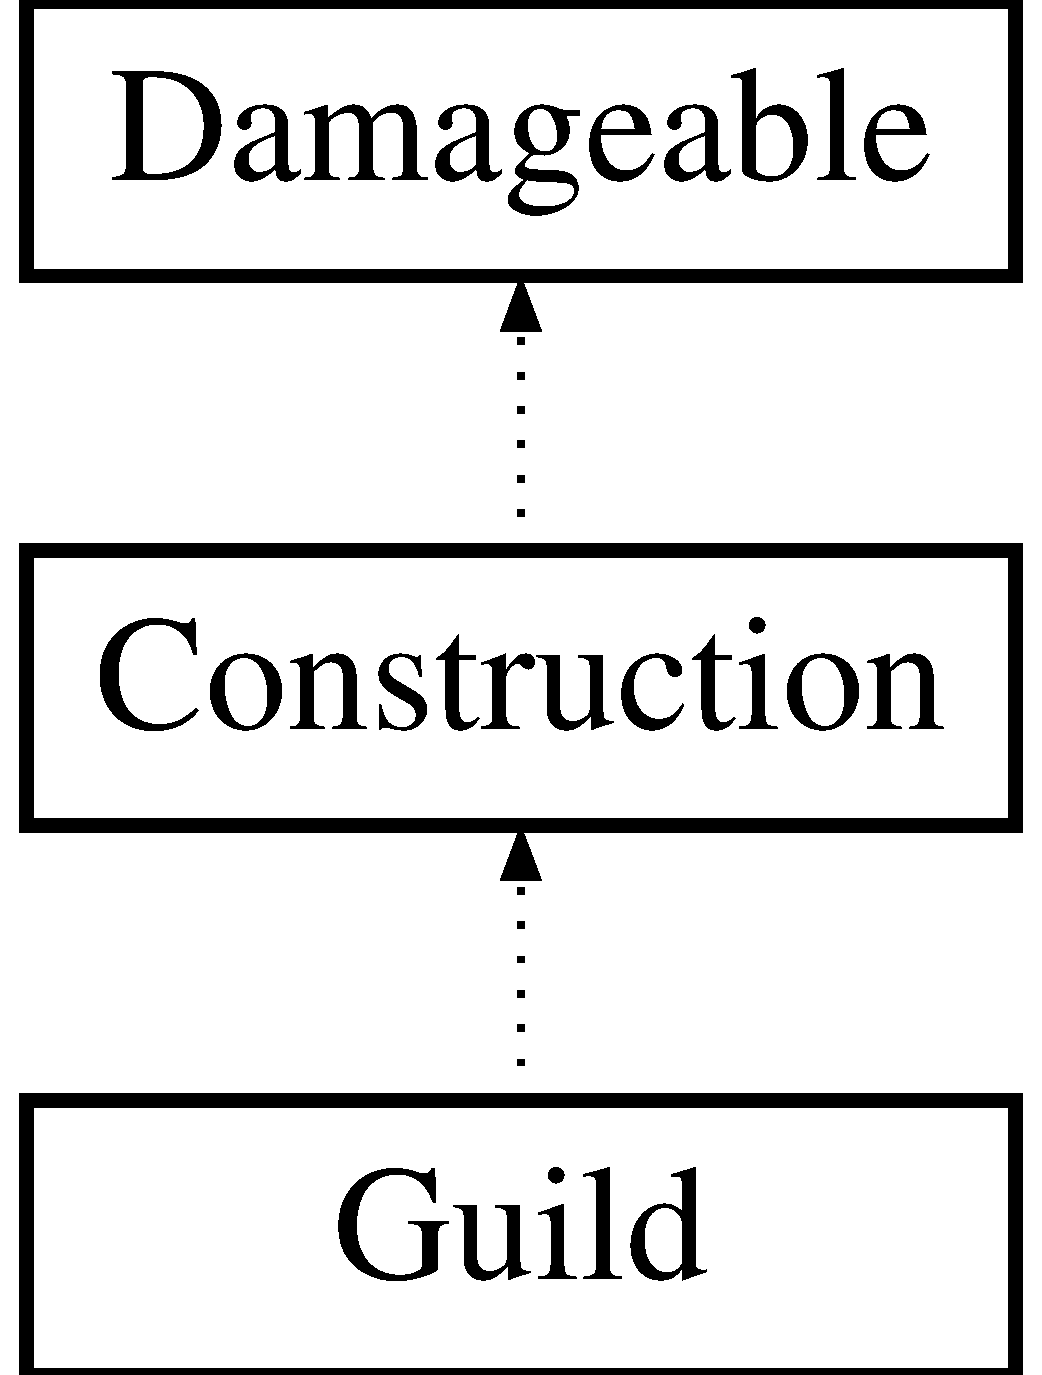
\includegraphics[height=3.000000cm]{class_construction}
\end{center}
\end{figure}
\subsection*{Protected Attributes}
\begin{DoxyCompactItemize}
\item 
string \hyperlink{class_construction_a1c41965939bcc09f9c55a6bb8f15b82e}{name}\hypertarget{class_construction_a1c41965939bcc09f9c55a6bb8f15b82e}{}\label{class_construction_a1c41965939bcc09f9c55a6bb8f15b82e}

\begin{DoxyCompactList}\small\item\em name of this \hyperlink{class_construction}{Construction} \end{DoxyCompactList}\end{DoxyCompactItemize}


\subsection{Detailed Description}
\hyperlink{class_construction}{Construction} standing in the World. 

\hyperlink{class_construction}{Construction} is either a Building owned by player or Lair of monsters 

The documentation for this class was generated from the following file\+:\begin{DoxyCompactItemize}
\item 
D\+:/proj\+\_\+majesty/\+Headers/Construction.\+h\end{DoxyCompactItemize}

\hypertarget{struct_mob_1_1damage}{}\section{Mob\+:\+:damage Struct Reference}
\label{struct_mob_1_1damage}\index{Mob\+::damage@{Mob\+::damage}}


how much damage this deals per attack. Keeps minimum and maxium amount  




{\ttfamily \#include $<$Mob.\+h$>$}

\subsection*{Public Attributes}
\begin{DoxyCompactItemize}
\item 
float {\bfseries min}\hypertarget{struct_mob_1_1damage_a998e416f7bf70858d8cf63c789b2d284}{}\label{struct_mob_1_1damage_a998e416f7bf70858d8cf63c789b2d284}

\end{DoxyCompactItemize}


\subsection{Detailed Description}
how much damage this deals per attack. Keeps minimum and maxium amount 

The documentation for this struct was generated from the following file\+:\begin{DoxyCompactItemize}
\item 
D\+:/proj\+\_\+majesty/\+Headers/Mob.\+h\end{DoxyCompactItemize}

\hypertarget{class_damageable}{}\section{Damageable Class Reference}
\label{class_damageable}\index{Damageable@{Damageable}}


Members of this class may be damaged.  




{\ttfamily \#include $<$Damageable.\+h$>$}

Inheritance diagram for Damageable\+:\begin{figure}[H]
\begin{center}
\leavevmode
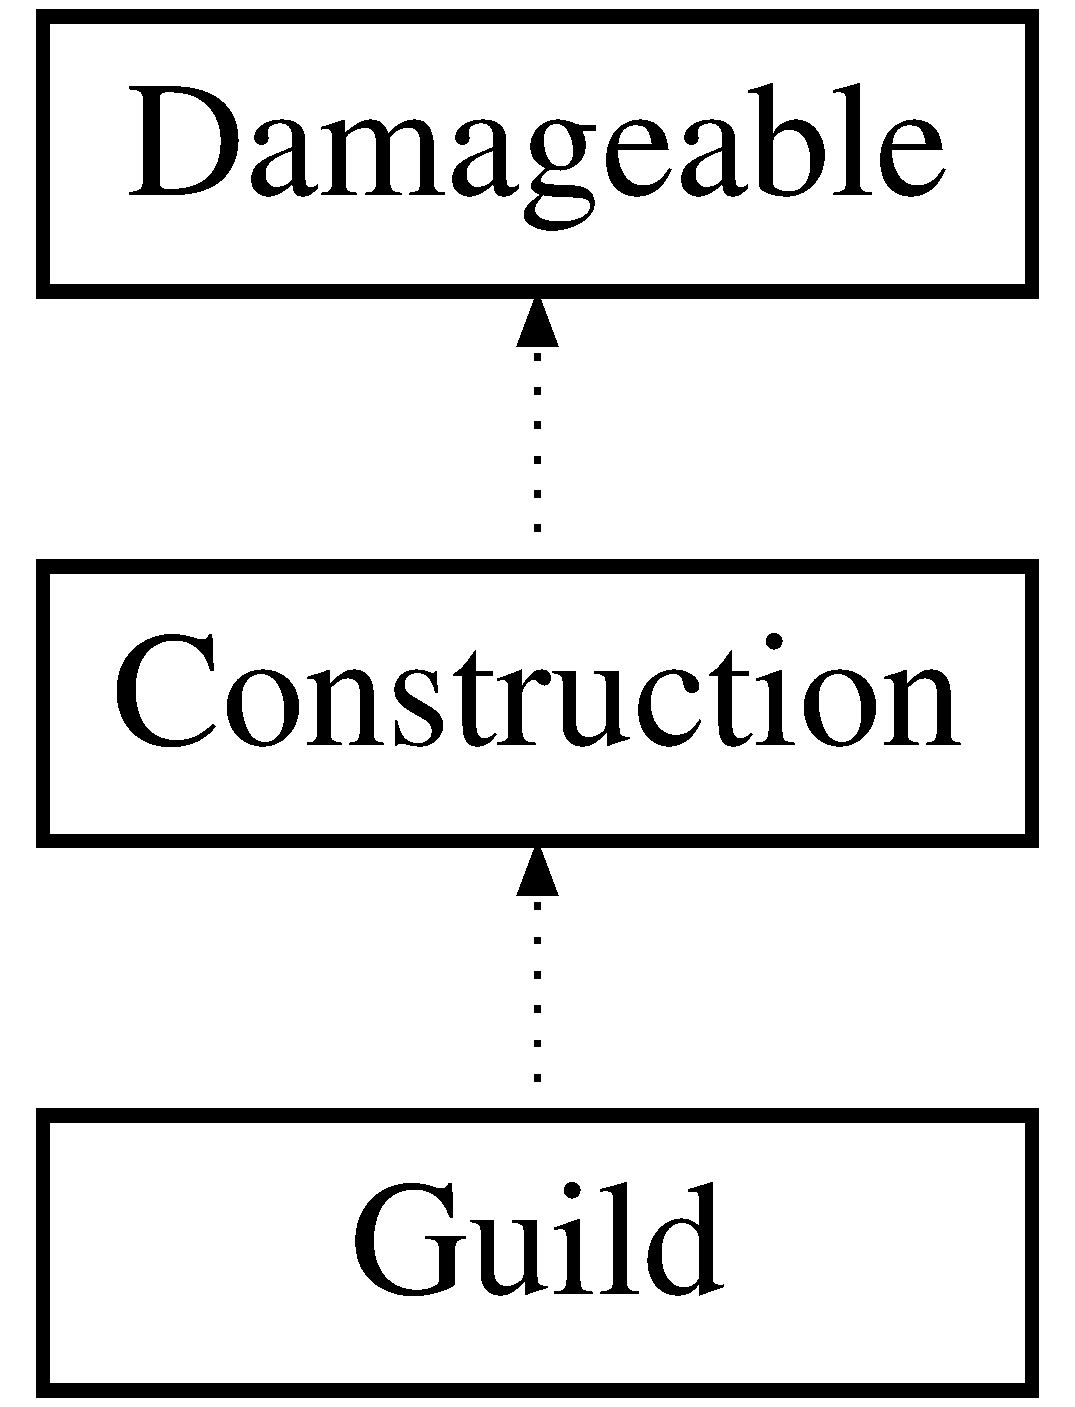
\includegraphics[height=3.000000cm]{class_damageable}
\end{center}
\end{figure}
\subsection*{Public Member Functions}
\begin{DoxyCompactItemize}
\item 
void \hyperlink{class_damageable_a61f6bcf8018bd7b126245f55ef29cd14}{die} ()\hypertarget{class_damageable_a61f6bcf8018bd7b126245f55ef29cd14}{}\label{class_damageable_a61f6bcf8018bd7b126245f55ef29cd14}

\begin{DoxyCompactList}\small\item\em give gold to mobs that killed this \hyperlink{class_mob}{Mob}, play death anim etc. \end{DoxyCompactList}\item 
bool \hyperlink{class_damageable_aa12cca043f17d936f5567fd08cd073af}{take\+Damage} (float pure\+Damage)\hypertarget{class_damageable_aa12cca043f17d936f5567fd08cd073af}{}\label{class_damageable_aa12cca043f17d936f5567fd08cd073af}

\begin{DoxyCompactList}\small\item\em reduce hp by amount of pure\+Damage reduced by this armor or skills, returns true if this died \end{DoxyCompactList}\end{DoxyCompactItemize}
\subsection*{Public Attributes}
\begin{DoxyCompactItemize}
\item 
float \hyperlink{class_damageable_a74600fde6cf8e5dcd88ddce654500496}{hp\+Current}\hypertarget{class_damageable_a74600fde6cf8e5dcd88ddce654500496}{}\label{class_damageable_a74600fde6cf8e5dcd88ddce654500496}

\begin{DoxyCompactList}\small\item\em how much hit points this has \end{DoxyCompactList}\item 
float \hyperlink{class_damageable_ac40b87477089440eff43ee438daa34d0}{hp\+Max}\hypertarget{class_damageable_ac40b87477089440eff43ee438daa34d0}{}\label{class_damageable_ac40b87477089440eff43ee438daa34d0}

\begin{DoxyCompactList}\small\item\em how much hit points this can have at max \end{DoxyCompactList}\item 
\hyperlink{class_mob}{Mob} $\ast$ \hyperlink{class_damageable_a2d91b79bfd5140c1cc62a2f7b96dd9f7}{threats}\hypertarget{class_damageable_a2d91b79bfd5140c1cc62a2f7b96dd9f7}{}\label{class_damageable_a2d91b79bfd5140c1cc62a2f7b96dd9f7}

\begin{DoxyCompactList}\small\item\em list of Mobs that damaged this \hyperlink{class_mob}{Mob} and should be rewarded for killing it \end{DoxyCompactList}\item 
int \hyperlink{class_damageable_a31f2ef8923b62447291f386807fccbab}{exp\+Reward}\hypertarget{class_damageable_a31f2ef8923b62447291f386807fccbab}{}\label{class_damageable_a31f2ef8923b62447291f386807fccbab}

\begin{DoxyCompactList}\small\item\em amount of experience that should be granted for killing this \end{DoxyCompactList}\item 
int \hyperlink{class_damageable_a29ecf4aca234318222ff32a33826656e}{gold\+Reward}\hypertarget{class_damageable_a29ecf4aca234318222ff32a33826656e}{}\label{class_damageable_a29ecf4aca234318222ff32a33826656e}

\begin{DoxyCompactList}\small\item\em amount of gold that should be granted for killing this \end{DoxyCompactList}\item 
int \hyperlink{class_damageable_ad5f2bf4daee7be1f1d673e0d5591dad0}{gold\+Carried}\hypertarget{class_damageable_ad5f2bf4daee7be1f1d673e0d5591dad0}{}\label{class_damageable_ad5f2bf4daee7be1f1d673e0d5591dad0}

\begin{DoxyCompactList}\small\item\em amount of gold carrier by this \end{DoxyCompactList}\item 
float \hyperlink{class_damageable_a7b4306631ce2d7dd8e50000b352940e4}{armor}\hypertarget{class_damageable_a7b4306631ce2d7dd8e50000b352940e4}{}\label{class_damageable_a7b4306631ce2d7dd8e50000b352940e4}

\begin{DoxyCompactList}\small\item\em how much damage this can resist each time it\textquotesingle{}s attacked \end{DoxyCompactList}\end{DoxyCompactItemize}


\subsection{Detailed Description}
Members of this class may be damaged. 

The documentation for this class was generated from the following file\+:\begin{DoxyCompactItemize}
\item 
D\+:/proj\+\_\+majesty/\+Headers/Damageable.\+h\end{DoxyCompactItemize}

\hypertarget{class_guild}{}\section{Guild Class Reference}
\label{class_guild}\index{Guild@{Guild}}


\hyperlink{class_guild}{Guild} is building that serves as home and school for Heros.  




{\ttfamily \#include $<$Guild.\+h$>$}

Inheritance diagram for Guild\+:\begin{figure}[H]
\begin{center}
\leavevmode
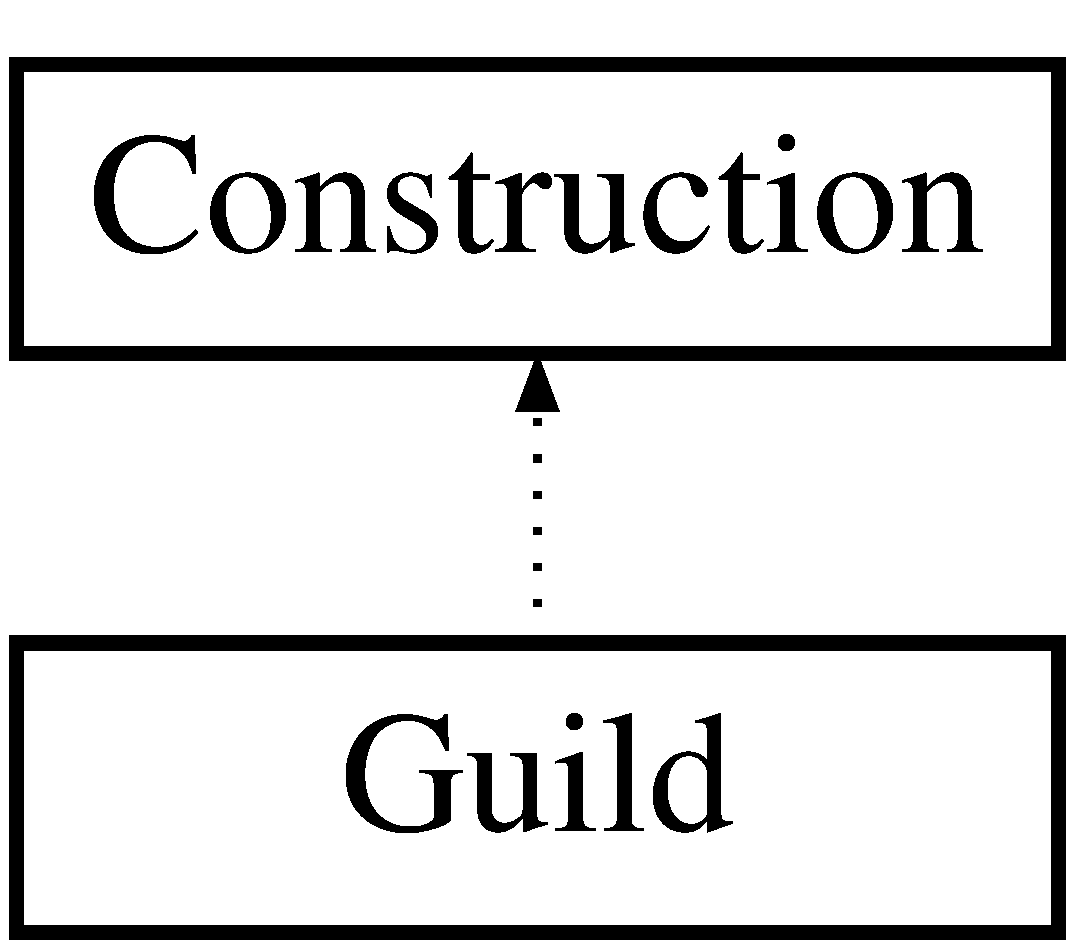
\includegraphics[height=2.000000cm]{class_guild}
\end{center}
\end{figure}
\subsection*{Public Member Functions}
\begin{DoxyCompactItemize}
\item 
void \hyperlink{class_guild_a5a671abed58577f1072bb3ce589d6f24}{spawn\+Hero} ()\hypertarget{class_guild_a5a671abed58577f1072bb3ce589d6f24}{}\label{class_guild_a5a671abed58577f1072bb3ce589d6f24}

\begin{DoxyCompactList}\small\item\em brings new \hyperlink{class_hero}{Hero} to live, adds him to list of habitants of this \hyperlink{class_guild}{Guild} \end{DoxyCompactList}\end{DoxyCompactItemize}
\subsection*{Protected Attributes}
\begin{DoxyCompactItemize}
\item 
\hyperlink{class_hero}{Hero} $\ast$ \hyperlink{class_guild_a96e8022f289bed1be880b03302d6de64}{hero\+Type}\hypertarget{class_guild_a96e8022f289bed1be880b03302d6de64}{}\label{class_guild_a96e8022f289bed1be880b03302d6de64}

\begin{DoxyCompactList}\small\item\em what kind of hero lives in this guild \end{DoxyCompactList}\end{DoxyCompactItemize}


\subsection{Detailed Description}
\hyperlink{class_guild}{Guild} is building that serves as home and school for Heros. 

\hyperlink{class_construction}{Construction} is either a Building owned by player or Lair of monsters 

The documentation for this class was generated from the following file\+:\begin{DoxyCompactItemize}
\item 
D\+:/proj\+\_\+majesty/\+Headers/Guild.\+h\end{DoxyCompactItemize}

\hypertarget{class_hero}{}\section{Hero Class Reference}
\label{class_hero}\index{Hero@{Hero}}


Independent individual seeking fame, gold or just advanture slaying beastes and compleating quests.  




{\ttfamily \#include $<$Hero.\+h$>$}

Inheritance diagram for Hero\+:\begin{figure}[H]
\begin{center}
\leavevmode
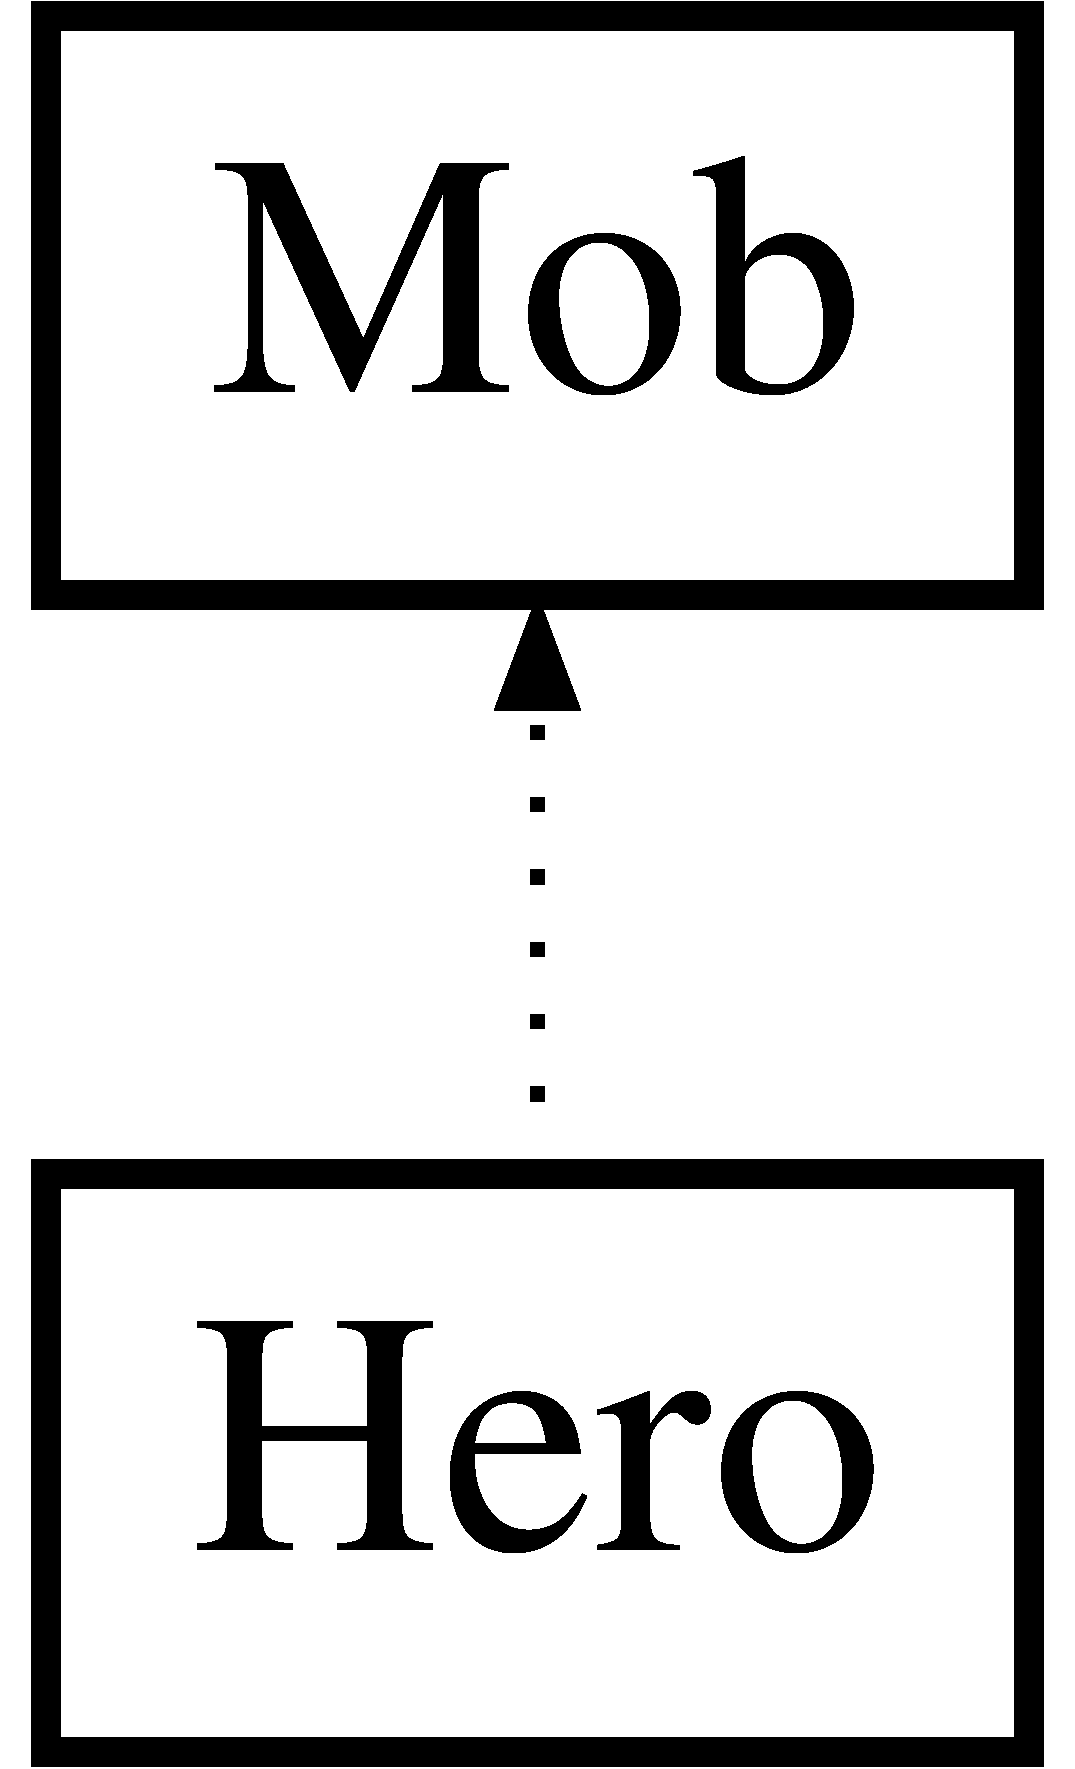
\includegraphics[height=2.000000cm]{class_hero}
\end{center}
\end{figure}


\subsection{Detailed Description}
Independent individual seeking fame, gold or just advanture slaying beastes and compleating quests. 

Heros are exceptional citizens of Player\textquotesingle{}s Kingdom, capable of facing threats on their own. 

The documentation for this class was generated from the following file\+:\begin{DoxyCompactItemize}
\item 
D\+:/proj\+\_\+majesty/\+Headers/Hero.\+h\end{DoxyCompactItemize}

\hypertarget{class_home}{}\section{Home Class Reference}
\label{class_home}\index{Home@{Home}}


Members of this class may be entered and be inhabited.  




{\ttfamily \#include $<$Home.\+h$>$}

\subsection*{Protected Attributes}
\begin{DoxyCompactItemize}
\item 
\hyperlink{class_mob}{Mob} $\ast$ \hyperlink{class_home_a09b567233eb88f856add661dbf49b11f}{inside}\hypertarget{class_home_a09b567233eb88f856add661dbf49b11f}{}\label{class_home_a09b567233eb88f856add661dbf49b11f}

\begin{DoxyCompactList}\small\item\em list of Mobs that are currently inside this \hyperlink{class_home}{Home} \end{DoxyCompactList}\item 
\hyperlink{class_mob}{Mob} $\ast$ \hyperlink{class_home_a04af272e407f5a688d269078ac942b67}{inhabitants}\hypertarget{class_home_a04af272e407f5a688d269078ac942b67}{}\label{class_home_a04af272e407f5a688d269078ac942b67}

\begin{DoxyCompactList}\small\item\em list of Mobs that usually lives in this \hyperlink{class_home}{Home} \end{DoxyCompactList}\end{DoxyCompactItemize}


\subsection{Detailed Description}
Members of this class may be entered and be inhabited. 

Interface for Constructions capable of giving shelter, like Monster\textquotesingle{}s Lair, Peasant\textquotesingle{}s hut or \hyperlink{class_hero}{Hero}\textquotesingle{}s \hyperlink{class_guild}{Guild} or an Inn(or maybe some kind of vechicles as well) 

The documentation for this class was generated from the following file\+:\begin{DoxyCompactItemize}
\item 
D\+:/proj\+\_\+majesty/\+Headers/Home.\+h\end{DoxyCompactItemize}

\hypertarget{class_mob}{}\section{Mob Class Reference}
\label{class_mob}\index{Mob@{Mob}}


Living form moving and taking actions in the World.  




{\ttfamily \#include $<$Mob.\+h$>$}

\subsection*{Public Member Functions}
\begin{DoxyCompactItemize}
\item 
bool \hyperlink{class_mob_af124fd088b64d10dde3eef2f5ec9f139}{take\+Damage} (float pure\+Damage)\hypertarget{class_mob_af124fd088b64d10dde3eef2f5ec9f139}{}\label{class_mob_af124fd088b64d10dde3eef2f5ec9f139}

\begin{DoxyCompactList}\small\item\em reduce hp by amount of pure\+Damage reduced by \hyperlink{class_mob}{Mob} armor or skills, returns true if \hyperlink{class_mob}{Mob} died \end{DoxyCompactList}\item 
void \hyperlink{class_mob_a07546ec7a5028846090157d51095904b}{die} ()\hypertarget{class_mob_a07546ec7a5028846090157d51095904b}{}\label{class_mob_a07546ec7a5028846090157d51095904b}

\begin{DoxyCompactList}\small\item\em give gold to mobs that killed you, play death anim etc. \end{DoxyCompactList}\item 
Goal \hyperlink{class_mob_ac949a1e6a9a60efd432adea5a4abdeb8}{decide\+What\+Next} ()\hypertarget{class_mob_ac949a1e6a9a60efd432adea5a4abdeb8}{}\label{class_mob_ac949a1e6a9a60efd432adea5a4abdeb8}

\begin{DoxyCompactList}\small\item\em after achieving goal think what\textquotesingle{}s your next goal(ie. if you completed quest either go rest if you are wounded or go to blacksmith to get better gear) \end{DoxyCompactList}\item 
Actor $\ast$ \hyperlink{class_mob_a80987418449007527dea30234099c301}{choose\+Target} ()\hypertarget{class_mob_a80987418449007527dea30234099c301}{}\label{class_mob_a80987418449007527dea30234099c301}

\begin{DoxyCompactList}\small\item\em choose Actor matching your goal(ie. if you are going to grind, find hostile \hyperlink{class_mob}{Mob} with low level and high reward, if you are going to upgrade find adequate shop, if rest -\/ nearest inn) \end{DoxyCompactList}\item 
void \hyperlink{class_mob_af89dfe24c4bea6d4fea6affd0b752c04}{interact} ()\hypertarget{class_mob_af89dfe24c4bea6d4fea6affd0b752c04}{}\label{class_mob_af89dfe24c4bea6d4fea6affd0b752c04}

\begin{DoxyCompactList}\small\item\em interact with target(while you are close enough) -\/ enter the building or hit an enemy \end{DoxyCompactList}\end{DoxyCompactItemize}
\subsection*{Protected Types}
\begin{DoxyCompactItemize}
\item 
enum \hyperlink{class_mob_a886346a9f913203df0797f2c84dd8962}{Goals} \{ \hyperlink{class_mob_a886346a9f913203df0797f2c84dd8962a3d18c0a90658cc4872eed0afe28790b4}{rest}, 
\hyperlink{class_mob_a886346a9f913203df0797f2c84dd8962aa72b321b37507255070e236e133616f9}{grind}, 
\hyperlink{class_mob_a886346a9f913203df0797f2c84dd8962a114d85e85d882dd8bf2be34208450b6c}{explore}, 
\hyperlink{class_mob_a886346a9f913203df0797f2c84dd8962ac9be3f62a039d2a4c5a63146a03a307d}{upgrade}
 \}\begin{DoxyCompactList}\small\item\em Goals enum. \end{DoxyCompactList}
\end{DoxyCompactItemize}
\subsection*{Protected Attributes}
\begin{DoxyCompactItemize}
\item 
string \hyperlink{class_mob_a1adcb405b2a4647bfb2471b1283b9477}{name}\hypertarget{class_mob_a1adcb405b2a4647bfb2471b1283b9477}{}\label{class_mob_a1adcb405b2a4647bfb2471b1283b9477}

\begin{DoxyCompactList}\small\item\em name of this mob \end{DoxyCompactList}\item 
\hyperlink{class_mob_a886346a9f913203df0797f2c84dd8962}{Goals} \hyperlink{class_mob_ad6c2e1b70a39551fd39b25002dac55b1}{goal}
\begin{DoxyCompactList}\small\item\em goal this \hyperlink{class_mob}{Mob} is trying to achieve, \end{DoxyCompactList}\item 
float {\bfseries hp\+Current}\hypertarget{class_mob_a5a84c7649f3774da15780caa9f21aabc}{}\label{class_mob_a5a84c7649f3774da15780caa9f21aabc}

\item 
float {\bfseries hp\+Max}\hypertarget{class_mob_ac2a881584e2fa3224da656a775f17284}{}\label{class_mob_ac2a881584e2fa3224da656a775f17284}

\item 
float {\bfseries mp\+Current}\hypertarget{class_mob_ae1388056fe541060e8c1607ae561801f}{}\label{class_mob_ae1388056fe541060e8c1607ae561801f}

\item 
float {\bfseries mp\+Max}\hypertarget{class_mob_a8156e952a713baa462990ce635bf9ae8}{}\label{class_mob_a8156e952a713baa462990ce635bf9ae8}

\item 
int \hyperlink{class_mob_a30bc4209cc6c6294cd3c68943317e682}{exp}\hypertarget{class_mob_a30bc4209cc6c6294cd3c68943317e682}{}\label{class_mob_a30bc4209cc6c6294cd3c68943317e682}

\begin{DoxyCompactList}\small\item\em how much this \hyperlink{class_mob}{Mob} has accumulated experience in it\textquotesingle{}s life. Important for leveling up \end{DoxyCompactList}\item 
Actor $\ast$ \hyperlink{class_mob_a1bf86299dea0aa82c773a3b8d04d0593}{target}\hypertarget{class_mob_a1bf86299dea0aa82c773a3b8d04d0593}{}\label{class_mob_a1bf86299dea0aa82c773a3b8d04d0593}

\begin{DoxyCompactList}\small\item\em \hyperlink{class_mob}{Mob} or \hyperlink{class_building}{Building} this mob is going to. \end{DoxyCompactList}\item 
\hyperlink{class_mob}{Mob} $\ast$ \hyperlink{class_mob_a07f79a9fd434b9b26098b3b6d5d4a93e}{threats}\hypertarget{class_mob_a07f79a9fd434b9b26098b3b6d5d4a93e}{}\label{class_mob_a07f79a9fd434b9b26098b3b6d5d4a93e}

\begin{DoxyCompactList}\small\item\em list of Mobs that damaged this \hyperlink{class_mob}{Mob} and should be rewarded for killing it \end{DoxyCompactList}\end{DoxyCompactItemize}


\subsection{Detailed Description}
Living form moving and taking actions in the World. 

\hyperlink{class_mob}{Mob} lives in world moving taking actions and interacting with another mobs and enviorment. Everybody from dire rat to king sitting in his throne room is a mob. 

\subsection{Member Enumeration Documentation}
\index{Mob@{Mob}!Goals@{Goals}}
\index{Goals@{Goals}!Mob@{Mob}}
\subsubsection[{\texorpdfstring{Goals}{Goals}}]{\setlength{\rightskip}{0pt plus 5cm}enum {\bf Mob\+::\+Goals}\hspace{0.3cm}{\ttfamily [protected]}}\hypertarget{class_mob_a886346a9f913203df0797f2c84dd8962}{}\label{class_mob_a886346a9f913203df0797f2c84dd8962}


Goals enum. 

This enum holds what\textquotesingle{}s in mind of the \hyperlink{class_mob}{Mob}. \begin{Desc}
\item[Enumerator]\par
\begin{description}
\index{rest@{rest}!Mob@{Mob}}\index{Mob@{Mob}!rest@{rest}}\item[{\em 
rest\hypertarget{class_mob_a886346a9f913203df0797f2c84dd8962a3d18c0a90658cc4872eed0afe28790b4}{}\label{class_mob_a886346a9f913203df0797f2c84dd8962a3d18c0a90658cc4872eed0afe28790b4}
}]\hyperlink{class_mob}{Mob} is tired or wounded and shall go home or to \char`\"{}sancturacy\char`\"{} to regain hp/mp or just to wait for something to happend \index{grind@{grind}!Mob@{Mob}}\index{Mob@{Mob}!grind@{grind}}\item[{\em 
grind\hypertarget{class_mob_a886346a9f913203df0797f2c84dd8962aa72b321b37507255070e236e133616f9}{}\label{class_mob_a886346a9f913203df0797f2c84dd8962aa72b321b37507255070e236e133616f9}
}]\hyperlink{class_mob}{Mob} is going to do it\textquotesingle{}s basic activity -\/ advanturer hunts, peasant works in a field and tax colector collects taxes \index{explore@{explore}!Mob@{Mob}}\index{Mob@{Mob}!explore@{explore}}\item[{\em 
explore\hypertarget{class_mob_a886346a9f913203df0797f2c84dd8962a114d85e85d882dd8bf2be34208450b6c}{}\label{class_mob_a886346a9f913203df0797f2c84dd8962a114d85e85d882dd8bf2be34208450b6c}
}]\hyperlink{class_mob}{Mob} is bored and is going to just walk around his home, it mind find something intrested, like treasure or death \index{upgrade@{upgrade}!Mob@{Mob}}\index{Mob@{Mob}!upgrade@{upgrade}}\item[{\em 
upgrade\hypertarget{class_mob_a886346a9f913203df0797f2c84dd8962ac9be3f62a039d2a4c5a63146a03a307d}{}\label{class_mob_a886346a9f913203df0797f2c84dd8962ac9be3f62a039d2a4c5a63146a03a307d}
}]\hyperlink{class_mob}{Mob(rather only advanturers)} has achieved enought wealth to upgrade it\textquotesingle{}s equipment or maybe change class \end{description}
\end{Desc}


\subsection{Member Data Documentation}
\index{Mob@{Mob}!goal@{goal}}
\index{goal@{goal}!Mob@{Mob}}
\subsubsection[{\texorpdfstring{goal}{goal}}]{\setlength{\rightskip}{0pt plus 5cm}{\bf Goals} Mob\+::goal\hspace{0.3cm}{\ttfamily [protected]}}\hypertarget{class_mob_ad6c2e1b70a39551fd39b25002dac55b1}{}\label{class_mob_ad6c2e1b70a39551fd39b25002dac55b1}


goal this \hyperlink{class_mob}{Mob} is trying to achieve, 

\begin{DoxySeeAlso}{See also}
\hyperlink{class_mob_a886346a9f913203df0797f2c84dd8962}{Goals} 
\end{DoxySeeAlso}


The documentation for this class was generated from the following file\+:\begin{DoxyCompactItemize}
\item 
D\+:/proj\+\_\+majesty/Mob.\+h\end{DoxyCompactItemize}

%--- End generated contents ---

% Index
\backmatter
\newpage
\phantomsection
\clearemptydoublepage
\addcontentsline{toc}{chapter}{Index}
\printindex

\end{document}
